\documentclass{beamer}
\beamertemplatenavigationsymbolsempty
\usecolortheme{beaver}
\setbeamertemplate{blocks}[rounded=true, shadow=true]
\setbeamertemplate{footline}[page number]
%
\usepackage[utf8]{inputenc}
\usepackage[english,russian]{babel}
\usepackage{amssymb,amsfonts,amsmath,mathtext}
\usepackage{subfig}
\usepackage[all]{xy} % xy package for diagrams
\usepackage{array}
\usepackage{multicol} % many columns in slide
\usepackage{hyperref} % urls
\usepackage{hhline} %tables
\usepackage{comment} %comments
\usepackage{adjustbox}
\usepackage{multirow}
\usepackage{booktabs}
\newcommand{\blambda}{\boldsymbol{\lambda}}
\newcommand{\e}{\varepsilon}
\newcommand{\R}{\mathbb{R}}
\newcommand{\E}{\mathbb{E}}
\DeclareMathOperator*{\argmin}{arg\,min}
\DeclareMathOperator*{\argmax}{arg\,max}
\usepackage{bm}

\usepackage{algorithm}
\usepackage{algorithmic}
%\usepackage{arxiv}
%\documentclass[12pt]{article}
%\usepackage[cp1251]{inputenc}
%\usepackage[russian]{babel}
\usepackage[utf8]{inputenc}
\usepackage[english, russian]{babel}
\usepackage[T2A, T1]{fontenc}
\usepackage{url}
\usepackage{booktabs}
\usepackage{amsfonts}
\usepackage{nicefrac}
\usepackage{microtype}
\usepackage{lipsum}
\usepackage{comment}
\usepackage{graphicx}
\usepackage{natbib}
\usepackage{doi}
\usepackage{hyperref}
\usepackage{amssymb, amsmath, latexsym}
% \usepackage{fullpage}
\usepackage{algorithm}
\usepackage{algorithmic}
%\usepackage{algpseudocode}
\usepackage{tabularx}
\usepackage{paralist}
\usepackage{mathtools}
%\usepackage{tcolorbox}
\usepackage{xcolor}
\usepackage{amsmath}


%\newtheorem{theorem}{Theorem}

% Your figures are here:
\graphicspath{ {../figures/} }

%----------------------------------------------------------------------------------------------------------

\title[Hamiltonian Monte Carlo]{Hamiltonian Monte Carlo Method for Sampling}
\author{Denis Rubtsov}
\institute{MIPT, Intelligence Systems Department}
\date{\today}

\begin{document}

%------------------------------------------------
\begin{frame}
  \titlepage
\end{frame}
%------------------------------------------------

\begin{frame}{Goal of the talk}
  \begin{itemize}
    \item Target: sample from a probability distribution on $\mathbb{R}^d$
    \[
      \pi(x) \propto e^{-f(x)}, \quad x \in \mathbb{R}^d,
    \]
    where $f$ is a potential (or negative log-density).
    \item This covers many Gibbs / Boltzmann distributions.
    \item Hamiltonian Monte Carlo (HMC) combines
      \begin{itemize}
        \item Markov chain Monte Carlo (MCMC),
        \item Hamiltonian dynamics from classical mechanics.
      \end{itemize}
    \item Idea: use physics-inspired dynamics to make \emph{long, informed} moves
          that still preserve the target distribution.
  \end{itemize}
\end{frame}
%------------------------------------------------

\begin{frame}{Motivation: why care about sampling?}
  \begin{itemize}
    \item Bayesian inference: posterior sampling for parameters and latent variables.
    \item Machine learning:
      \begin{itemize}
        \item training and uncertainty estimation in complex models,
        \item approximate integration, model averaging, Bayesian model selection.
      \end{itemize}
    \item Physics and chemistry:
      \begin{itemize}
        \item molecular dynamics, Ising models, reaction rates, material design.
      \end{itemize}
    \item Optimization:
      \begin{itemize}
        \item escaping local minima / saddle points,
        \item robust training in non-convex landscapes.
      \end{itemize}
  \end{itemize}
\end{frame}
%------------------------------------------------

\begin{frame}{Classical MCMC and its limitations}
  \textbf{Random-walk Metropolis / Ball walk}
  \begin{itemize}
    \item Propose
      \[
        \tilde X_{i+1} = X_i + \eta V_i,
      \]
      where $V_i$ is isotropic noise (e.g. Gaussian).
    \item Accept with probability
      \[
        \alpha = \min\left(1,\;\frac{\pi(\tilde X_{i+1})}{\pi(X_i)}\right).
      \]
  \end{itemize}
  Problems:
  \begin{itemize}
    \item Step size $\eta$ must be small to keep acceptance reasonable.
    \item In high dimensions, random walk explores space slowly
          (diffusive behaviour, mixing time often scales at least like $d$).
  \end{itemize}
  \end{frame}
  
\begin{frame}{Classical MCMC and its limitations}
  \vspace{0.2cm}
  \textbf{Langevin algorithms}
  \begin{itemize}
    \item Use gradient information:
      \[
        X_{i+1} = X_i - \eta \nabla f(X_i) + \sqrt{2\eta}\,V_i.
      \]
    \item Improvement over pure random walk, but “momentum” is lost after each step.
  \end{itemize}
\end{frame}
%------------------------------------------------

\begin{frame}{Hamiltonian dynamics}
  Consider a particle of unit mass with
  \begin{itemize}
    \item position $x \in \mathbb{R}^d$,
    \item velocity (momentum) $v \in \mathbb{R}^d$.
  \end{itemize}
  Define the \textbf{Hamiltonian}
  \[
    H(x,v) = f(x) + \frac{1}{2}\|v\|^2,
  \]
  where $f(x)$ plays the role of potential energy.

  \vspace{0.2cm}
  \textbf{Hamilton’s equations}
  \[
    \frac{dx}{dt} = \frac{\partial H}{\partial v} = v,
    \qquad
    \frac{dv}{dt} = -\frac{\partial H}{\partial x} = -\nabla f(x).
  \]

  The solution at time $t$ starting from $(x,v)$ is denoted
  \[
    \varphi_t(x,v) = (x_t(x,v), v_t(x,v)),
  \]
  the \emph{Hamiltonian flow}.
\end{frame}
%------------------------------------------------

\begin{frame}{Key properties of Hamiltonian dynamics}
  For the dynamics defined by $H(x,v) = f(x) + \frac{1}{2}\|v\|^2$:
  \begin{itemize}
    \item \textbf{Energy conservation:}
      \[
        H(x_t, v_t) = H(x_0, v_0) \quad \forall t.
      \]
    \item \textbf{Volume preservation in phase space:}
      \begin{itemize}
        \item The flow $\varphi_t$ has Jacobian determinant 1,
              i.e.\ it preserves Lebesgue measure on $(x,v)$ space.
      \end{itemize}
    \item \textbf{Time reversibility:}
      \[
        \varphi_t(x_t, -v_t) = (x_0, -v_0),
      \]
      so dynamics can be run forward or backward.
  \end{itemize}

  \vspace{0.2cm}
  These properties are crucial: they allow us to build Markov transitions
  that preserve a desired joint density on $(x,v)$.
\end{frame}
%------------------------------------------------
\begin{frame}{Example}
\begin{figure}
    \centering
    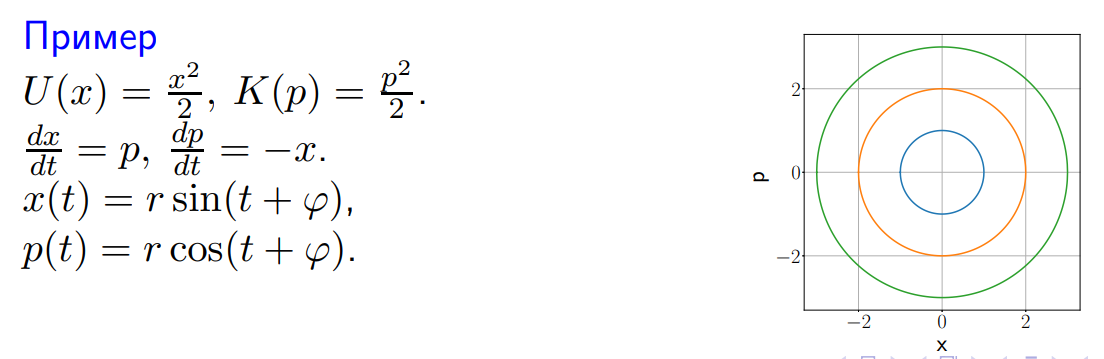
\includegraphics[width=0.9\textwidth]{example.png}
\end{figure}
\end{frame}
%------------------------------------------------

\begin{frame}{Extended target distribution}
  Define a joint density on position $x$ and momentum $v$:
  \[
    \pi(x,v) \propto \exp\big(-H(x,v)\big)
    = \exp\left(-f(x) - \frac{1}{2}\|v\|^2\right).
  \]
  Then:
  \begin{itemize}
    \item The conditional distribution of $v$ given $x$ is
      \[
        v \mid x \sim \mathcal{N}(0, I_d).
      \]
    \item Marginalizing over $v$ gives
      \[
        \pi(x) \propto e^{-f(x)},
      \]
      which is our target density.
    \item Under exact Hamiltonian dynamics, the density $\pi(x,v)$ is \emph{invariant}:
      \[
        (X,V) \sim \pi \quad\Rightarrow\quad \varphi_T(X,V) \sim \pi
        \quad \forall T \ge 0.
      \]
  \end{itemize}
\end{frame}
%------------------------------------------------

\begin{frame}{Idealized Hamiltonian Monte Carlo}
  \textbf{Algorithm (idealized HMC with exact integration)}
  \begin{enumerate}
    \item Start at $X_0 \in \mathbb{R}^d$.
    \item For $i = 1,2,\dots,k$:
      \begin{enumerate}
        \item Sample a fresh momentum
          \[
            \xi_i \sim \mathcal{N}(0, I_d).
          \]
        \item Run Hamiltonian dynamics for time $T$:
          \[
            (X_i, V_i) = \varphi_T(X_{i-1}, \xi_i).
          \]
      \end{enumerate}
  \end{enumerate}

  \vspace{0.2cm}
  \textbf{Properties}
  \begin{itemize}
    \item The Markov chain $(X_i, V_i)$ has invariant density $\pi(x,v)$.
    \item The marginal chain $(X_i)$ has invariant density $\pi(x)$.
    \item No Metropolis correction is needed if we integrate exactly.
  \end{itemize}
\end{frame}
%------------------------------------------------

\begin{frame}{Why does idealized HMC preserve $\pi(x,v)$?}
  Sketch of argument:
  \begin{itemize}
    \item Start from $(X,V) \sim \pi(x,v) \propto e^{-H(x,v)}$.
    \item Along the trajectory $(x_t,v_t)$,
      \[
        H(x_t,v_t) = H(x_0,v_0),
      \]
      so the value of $e^{-H}$ is constant on orbits.
    \item The flow $\varphi_T$ preserves phase-space volume
          (Jacobian determinant $=1$).
    \item Therefore, the push-forward of $\pi$ under $\varphi_T$ is again $\pi$.
  \end{itemize}

  \vspace{0.2cm}
  Conclusion:
  \begin{itemize}
    \item Any map that is energy-preserving and volume-preserving leaves
          $\pi(x,v) \propto e^{-H(x,v)}$ invariant.
    \item Resampling momentum from $\mathcal{N}(0,I_d)$ between trajectories
          also preserves the marginal $v$-distribution.
  \end{itemize}
\end{frame}
%------------------------------------------------

\begin{frame}{Convergence for strongly log-concave targets}
  Assume:
  \begin{itemize}
    \item $f$ is twice differentiable.
    \item $f$ is $m$-strongly convex and $M$-smooth:
      \[
        mI \preceq \nabla^2 f(x) \preceq MI \quad \forall x.
      \]
  \end{itemize}
  Then for idealized HMC with appropriate integration time $T$:
  \begin{itemize}
    \item The distance between their positions contracts geometrically in
          Wasserstein distance:
      \[
        W_2(\nu_k, \pi) \le C (1-\gamma)^k,
      \]
      for constants $C$ and $\gamma$ depending on $m,M$.
    \item With $T = \Theta\!\left(\sqrt{m/M}\right)$ the number of steps
          to reach error $\varepsilon$ is
          \[
            k = \mathcal{O}\!\left(\left(\frac{M}{m}\right)^2 \log \frac{1}{\varepsilon}\right),
          \]
          and can be improved to linear in $M/m$ in sharper analyses.
  \end{itemize}
\end{frame}
%------------------------------------------------

\begin{frame}{Discretizing Hamiltonian dynamics}
  In practice we cannot solve Hamilton’s ODEs exactly.
  We use a numerical integrator, typically \textbf{leapfrog}:
  \[
  \begin{aligned}
    v_{t+\frac{\varepsilon}{2}} &= v_t - \frac{\varepsilon}{2}\nabla f(x_t), \\
    x_{t+\varepsilon} &= x_t + \varepsilon v_{t+\frac{\varepsilon}{2}}, \\
    v_{t+\varepsilon} &= v_{t+\frac{\varepsilon}{2}}
      - \frac{\varepsilon}{2}\nabla f(x_{t+\varepsilon}),
  \end{aligned}
  \]
  where $\varepsilon$ is a step size.

  \vspace{0.2cm}
  Properties of leapfrog:
  \begin{itemize}
    \item Second-order accurate: error over time $T = L\varepsilon$
          is $\mathcal{O}(T\varepsilon^2)$.
    \item Time reversible.
    \item Symplectic: approximately preserves phase-space volume and
          a modified Hamiltonian.
  \end{itemize}
\end{frame}
%------------------------------------------------

\begin{frame}{Practical HMC algorithm (with Metropolis step)}
  \textbf{Input:} current position $x$, step size $\varepsilon$, number of steps $L$.
  \begin{enumerate}
    \item Sample momentum $p \sim \mathcal{N}(0,I_d)$.
    \item Set $(x^{(0)},p^{(0)}) = (x,p)$.
    \item Apply $L$ leapfrog steps with step size $\varepsilon$ to obtain
          $(x^{(L)}, p^{(L)})$.
    \item Negate momentum: $\tilde p = -p^{(L)}$ (for reversibility).
    \item Accept $(x',p')=(x^{(L)},\tilde p)$ with probability
      \[
        \alpha = \min\Big(1,\;
          \exp\big(-H(x',p') + H(x,p)\big)\Big).
      \]
      Otherwise keep $(x',p')=(x,p)$.
    \item Output new position $x'$ and discard momentum.
  \end{enumerate}
\end{frame}
%------------------------------------------------

\begin{frame}{Tuning and comparison}
  \textbf{Tuning parameters}
  \begin{itemize}
    \item Step size $\varepsilon$:
      \begin{itemize}
        \item too large $\Rightarrow$ high discretization error, low acceptance;
        \item too small $\Rightarrow$ expensive trajectories.
      \end{itemize}
    \item Number of leapfrog steps $L$ or total integration time $T = L\varepsilon$.
    \item Mass matrix (covariance of momentum) can be adapted to geometry.
  \end{itemize}

  \vspace{0.2cm}
  \textbf{Advantages over random-walk / Gibbs / Langevin}
  \begin{itemize}
    \item Uses gradients and momentum to move \emph{ballistically} rather than diffusively.
    \item Can traverse long distances in state space while maintaining high acceptance.
    \item Better scaling in high dimensions for many problems.
  \end{itemize}
\end{frame}
%------------------------------------------------

\begin{frame}{Summary}
  \begin{itemize}
    \item HMC augments position $x$ with momentum $v$ and simulates Hamiltonian dynamics
          to propose distant, high-probability moves.
    \item Exact Hamiltonian flow preserves the extended density
          $\pi(x,v) \propto \exp(-H(x,v))$, hence the target $\pi(x)$.
    \item For strongly convex and smooth $f$, the idealized HMC chain converges
          rapidly in Wasserstein distance.
    \item In practice, leapfrog integration + Metropolis correction yields
          an efficient and widely used sampler (e.g.\ in Stan).
  \end{itemize}
\end{frame}
%------------------------------------------------

 
\end{document}
